\documentclass{beamer}
\usepackage{upgreek}
\usepackage{amsmath}
\usepackage{array}
\usepackage{bm}

\usetheme[]{POSTERen}
\newcommand{\bb}[1]{\mathbf{#1}}

\begin{document}

\begin{frame}
\justifying 

\begin{columns}
\begin{column}{0.05\paperwidth}
\end{column}
\begin{column}{0.425\paperwidth}
\justifying 

\begin{textblock}{17.8}(2.1,1.5)

\begin{center} 
{\Large Bachelor thesis}

\vskip0.75cm
{\LARGE \textbf{Dynamic analysis of planar multibody systems based on Hamilton's canonical coordinates}}

\vskip1cm
{\Large Wojciech Celej}

{\large Automatic Control and Robotics}

{\large Robotics}

{Academic year 2017/2018}

\vskip0.5cm
{\large Supervisor: dr inż. Paweł Malczyk}
\vskip1cm
\end{center} 
\end{textblock}

\vskip6.5cm

{\Large 1. Introduction}
\vskip8pt 

Main purpose of the thesis is to create universal solver for the forward dynamic simulation of planar multibody systems. In order to do that, various formulations were tested and canonical coordinates were selected. To avoid solving differntial-algebraic equations, penalty method was implemented (with $\alpha$, $\xi$ and $\omega$ as penalty factors). Therefore, canonical equations of motion based on augmented Lagrangian and Hamiltonian can be presented as below:

\begin{align} \label{eq1}
(&\bb{M} + \bb{\Phi}_\bb{q}^T \alpha \bb{\Phi}_\bb{q})\bb{\dot{q}} = \bb{p} -\bb{\Phi}_\bb{q}^T \alpha \left(2\xi \omega \bb{\Phi} + \omega^2 \int_{t_0}^{t}\bb{\Phi} d\tau \right) - \bb{\Phi}_\bb{q}^T \bm{\widetilde{\upsigma}} \\ \label{eq2}
&\bb{\dot{p}}=\bb{Q} + \bb{\dot{\Phi}}_\bb{q}^T \alpha \left( \bb{\dot{\Phi}} + 2\xi\omega \bb{\Phi} + \omega^2 \int_{t_0}^{t}\bb{\Phi} d\tau \right) + \bb{\dot{\Phi}}_\bb{q}^T \bm{\widetilde{\upsigma}} \\
&\bm{\upsigma}=\bm{\widetilde{\upsigma}}+\alpha \left(\bb{\dot{\Phi}} + 2\xi \omega \bb{\Phi} + \omega^2 \int_{t_0}^{t}\bb{\Phi} d\tau \right)
\end{align}

With $\bb{q}$ (generalized coordinates), $\bb{p}$ (canonical momenta) and $\bm{\upsigma}$ (Lagrange's multipliers) as unknown. Those equations are applied to Andrew's squeezer mechanism (that is an example of stiff mechanism - including high and low frequencies in response). Figures below present mechanism's structure and solver's results (point F position during 0.05 s simulation).

\begin{figure}
\centering
\begin{minipage}{0.38\textwidth}
  \centering
 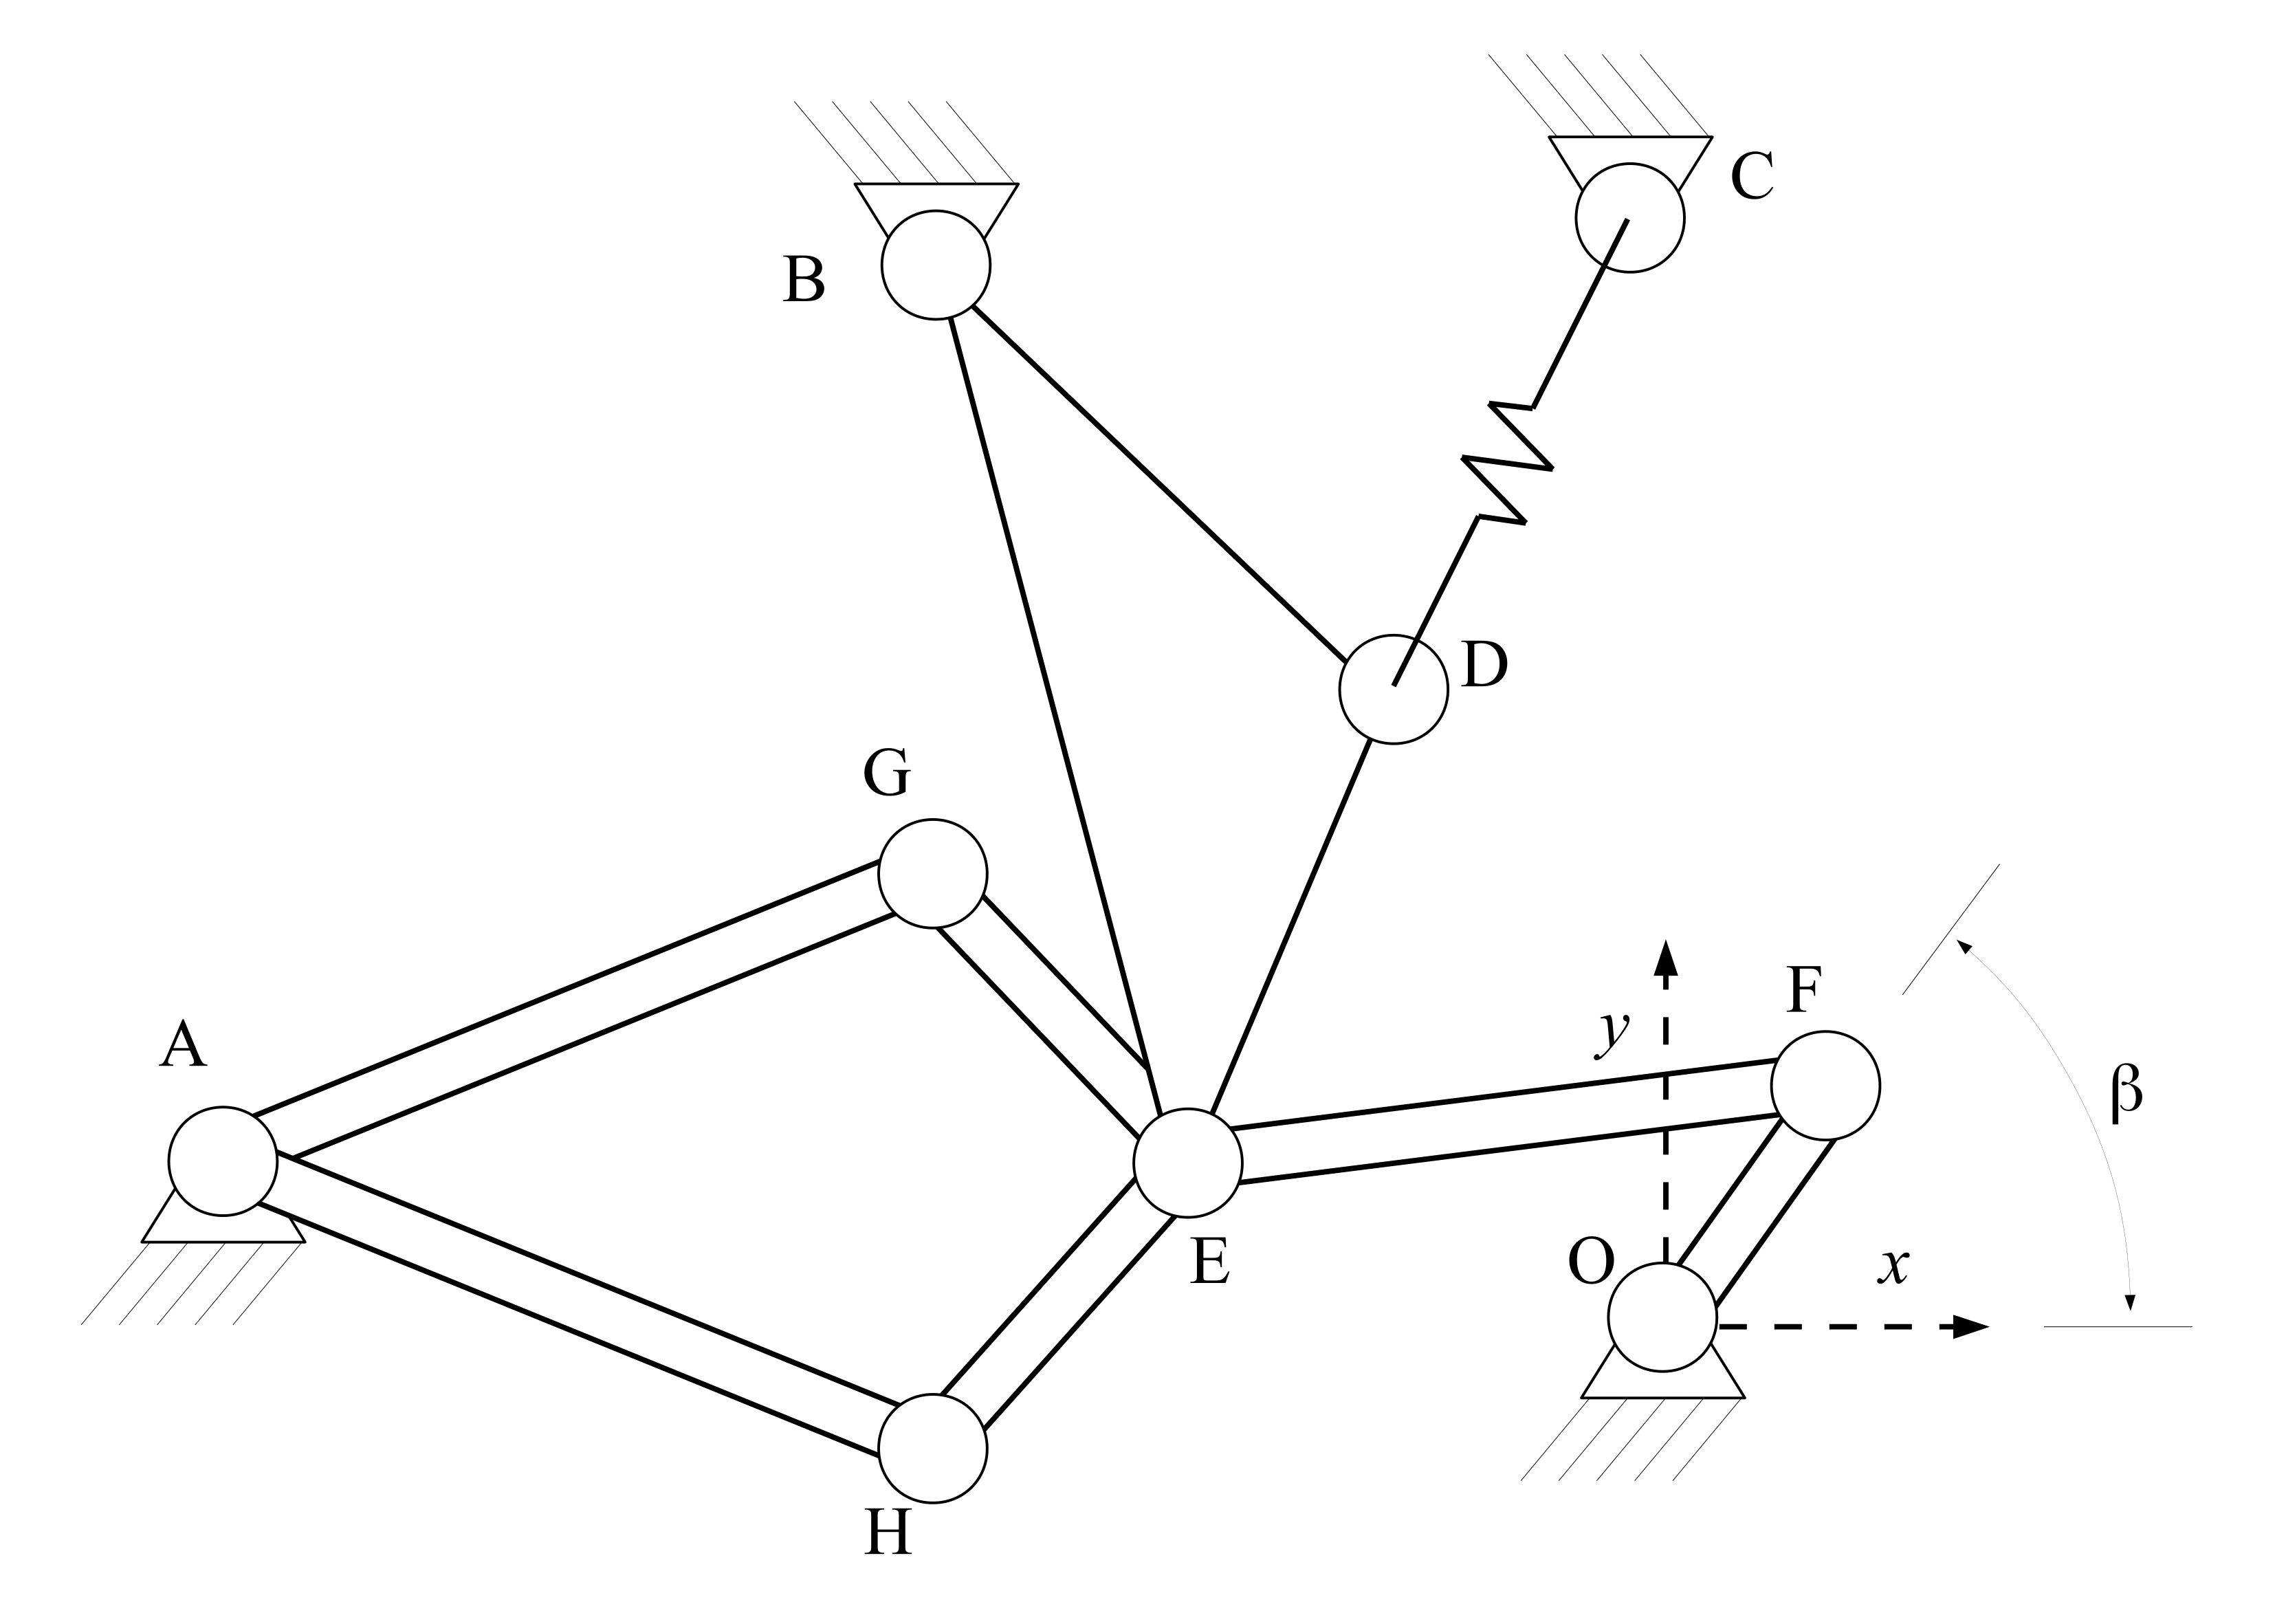
\includegraphics[width=\textwidth]{Andrews_mech}
\caption{Andrew's squeezer mechanism}
  \label{fig:test1}
\end{minipage}%
\begin{minipage}{0.62\textwidth}
  \centering
\includegraphics[width=\textwidth]{Position_F}
\caption{Time history of the x and y coordinates of point F}
\end{minipage}
\end{figure}


\end{column}
\begin{column}{0.05\paperwidth}
\end{column}
\begin{column}{0.425\paperwidth}
\justifying

\vskip6pt 
{\Large 2. Comparison between explicit and implicit integrator}
\vskip6pt 

\emph{Ode45} (based on Runge-Kutta methods Matlab's procedure) was selected as representative of explicit integrator. Subsequently trapezoidal rule (implicit, A-stable integrator) was used. The expression of the trapezoidal rule applied to equations (\ref{eq1}) and (\ref{eq2}) can be presented as:
\begin{align}
\bb{\dot{q}}_{k+1}=\dfrac{2}{h}(\bb{q}_{k+1}-\bb{q}_k)-\bb{\dot{q}}_k, \qquad \bb{\dot{p}}_{k+1}=\dfrac{2}{h}(\bb{p}_{k+1}-\bb{p}_k)-\bb{\dot{p}}_k
\end{align}

In consequence, a set of non-linear equations must be solved in each iteration (using Newton-Raphson method). Comparison between those two integrators is presented in the context of constraint violation errors and total energy conservation (on  Andrew's mechanism example). 

\begin{figure}
\centering
\begin{minipage}{0.5\textwidth}
  \centering
 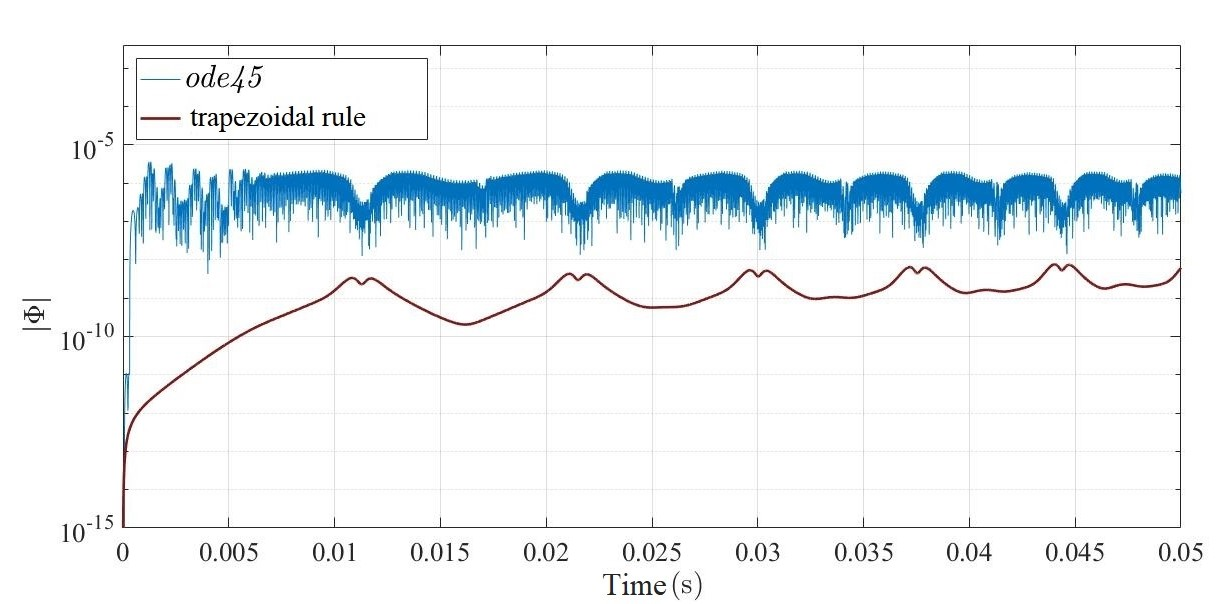
\includegraphics[width=\textwidth]{Phi_comp_1}
\caption{Constraint violation for coordinates $\bb{q}$}
  \label{fig:test1}
\end{minipage}%
\begin{minipage}{0.5\textwidth}
  \centering
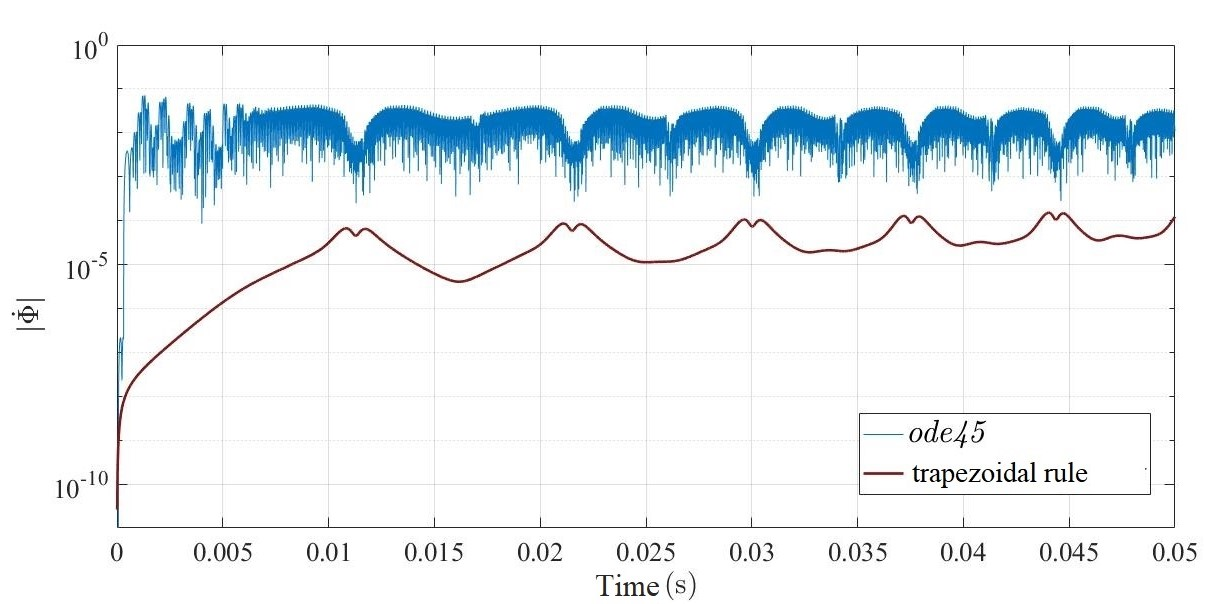
\includegraphics[width=\textwidth]{dPhi_comp_1}
\caption{Constraint violation for velocities $\bb{\dot{q}}$}
\end{minipage}
\end{figure}
\begin{columns}
\begin{column}{0.5\textwidth}
\begin{figure}
\centering
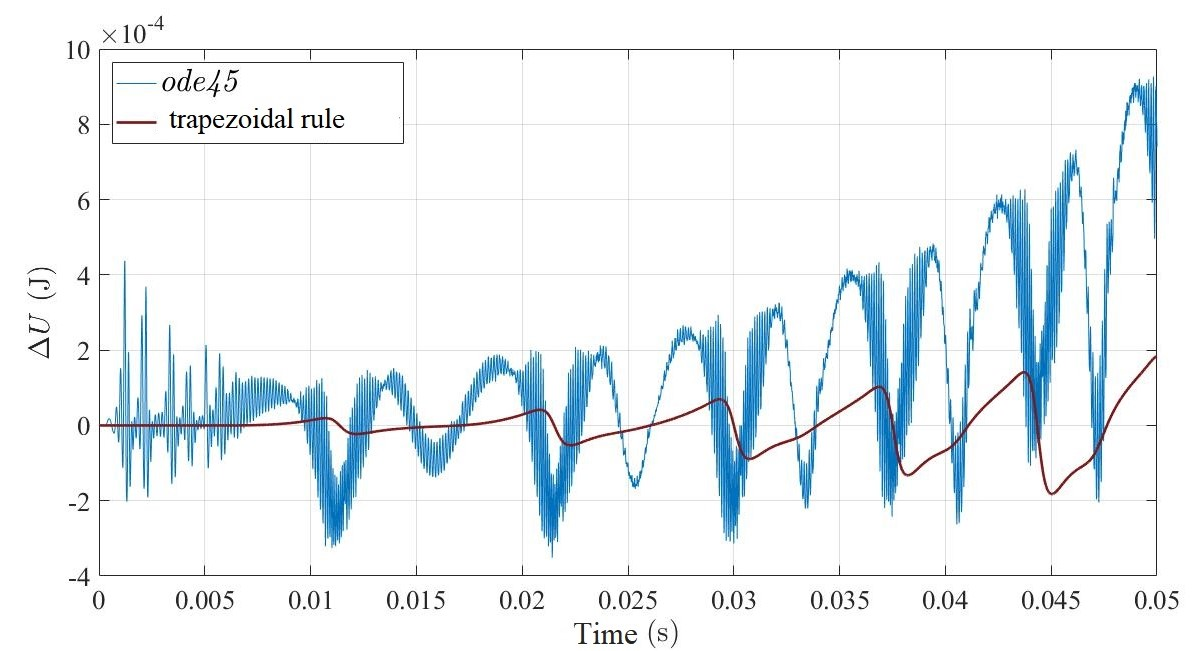
\includegraphics[width=\textwidth]{E_comp_1}
\caption{Total energy violation}
\end{figure}
\end{column}

\begin{column}{0.4\textwidth}
\centering
\begin{block}{\emph{A-stability}}
means that the numerical solution decays to zero whenever the corresponding exact solution decays to zero
\end{block}

\end{column}
\end{columns}

\vskip8pt
{\Large 3. Conclusions}
\vskip6pt

\begin{itemize}
\item Formulation based on canonical equations and augmented Lagrangian (with trapezoidal rule as integrator) deals with stiff systems (moreover with singular configurations, intermittent motion, dependent constraints) hence that is suitable for universal solvers.
\item Trapezoidal rule is more accurate and stable in the context of constraint violation and energy conservation (regardless of stabilization parameters).
\item Trapezoidal rule is energy preserving while explicit methods tend to increase total energy.
\item \emph{A-stable} methods are dedicated to integrate stiff systems (it is possible to integrate even with larger time step and keep accuracy on sufficient level).
\end{itemize} 

\end{column}
\begin{column}{0.05\paperwidth}
\end{column}
\end{columns}
\end{frame}

\end{document}